\chapter{Basics of RADAR (RAdio Detection And Ranging)}
	The electromagnetic waves are reflected if they meet an electrically leading surface. If these reflected waves are received again at the place of their origin, then that means an obstacle is in the propagation direction. Electromagnetic energy travels through air at a constant speed, at approximately the speed of light. This energy normally travels through space in a straight line, and will vary only slightly because of atmospheric and weather conditions. By using of special radar antennas this energy can be focused into a desired direction. Thus the direction (in azimuth and elevation) of the reflecting objects can be measured. These principles can basically be implemented in a radar system, and allow the determination of the distance, the direction and the height of the reflecting object.
	
Radar units usually work with very high frequencies. Reasons for this are:
\begin{itemize}
\item quasi-optically propagation of these waves.
\item High resolution (the smaller the wavelength, the smaller the objects the radar is able to detect).
\item Higher the frequency, smaller the antenna size at the same gain.
\end{itemize}

\section{Advantages}
Radar has many advantages compared to an attempt of visual observation:
\begin{itemize}
\item Radar is able to operate day or night, in lightness or darkness over a long range;
\item Radar is able to operate in all weathers, in fog and rain, it can even penetrate walls or layers of snow;
\item Radar has very broad coverage; it is possible to observe the whole hemisphere;
\item Radar detects and tracks moving objects, a high resolution imaging is possible, that results in an object recognition;
\item Radar can operate unmanned, 24 hours a day, 7 days a week.
\end{itemize}

\section{Miniature FMCW Radar}

\begin{figure}
\centering
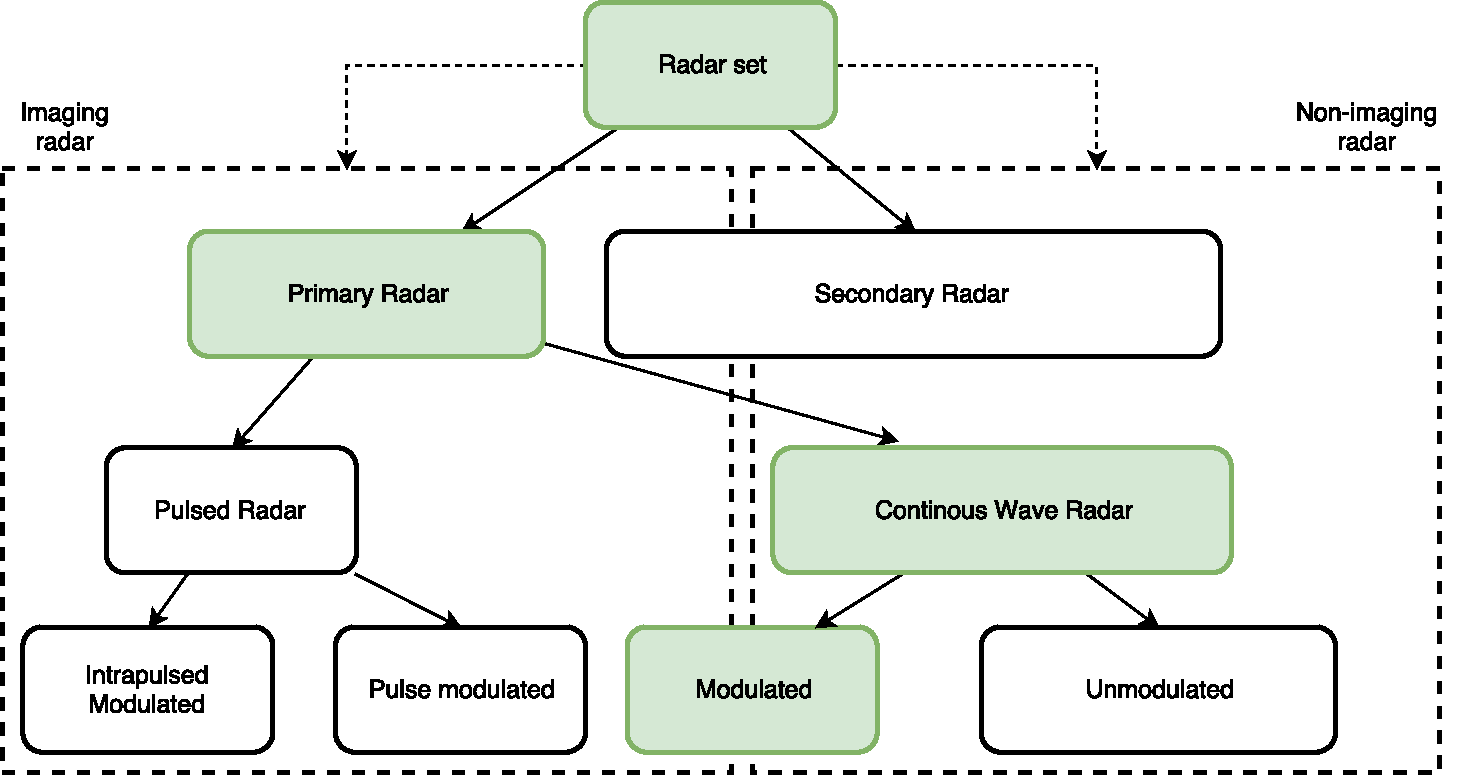
\includegraphics[width = 6in]{radar_classification.pdf}
\caption{Radar classification (The project belongs to the highlighted category)}
\end{figure}	

The configuration of radar is bistatic.
\section{Signal Processing}
		\subsection{Brief} The signal processing chain starts from the IF amplifier. An ADC samples the IF signal and send the data to the FPGA (DSP). The FPGA is the Cyclone V SoC from Intel (Altera). The FPGA performs the real time FFT to provide the frequency components.
		\subsection{Transmitter stage}
		The power amplifier is responsible for providing maximum power to the antenna. Unfortunately due to certain factors like antenna gain, impedance mismatch, and other losses which are related to antenna efficiency (conduction losses, dielectric losses).	
		The phase noise of the VCO should be as minimum as possible for better resolution. If not so then the phase noise tail would corrupt the wanted signal reflected back from the target.
		
\begin{figure}
\centering
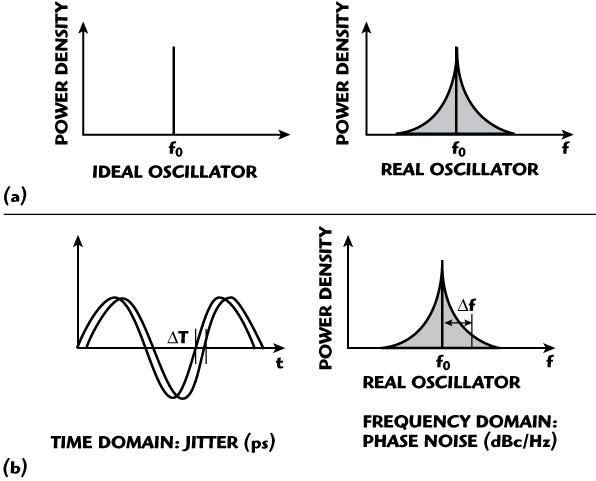
\includegraphics[width=4in]{Synergy_Microwave_Corporation_Jitter_and_Phase_Noise.jpg}
\caption{Phase noise and jitter}
Source : Synergy Microwave Corporation
\end{figure} 

		\subsection{Receiver stage}
		Typical received signal power is found to be around -150dBm to -30dBm. So these are needed to be amplified before being fed into mixer. A low noise amplifier is required for this purpose. 
		Phase noise is a key parameter for transceivers
		\subsection{IF amplifier stage}
		Bandwidth B, BW or $\Delta{f}$ is the difference between the upper and lower cut-off frequencies of a radar receiver, and is typically measured in hertz. In case of a baseband channel or video signal, the bandwidth is equal to its upper cut-off frequency. In a Radar receiver the bandwidth is mostly determined by the IF filter stages. The receiver must be able to process the signal bandwidth of the backscattered electromagnetic radiation from target.
The wider the bandwidth, the greater the degree of noise that will be input to the receiver. Since noise exists at all frequencies, the broader the frequency range to which the receiver bandpass filters are tuned, then the higher the intensity level of the noise and the lower the signal-to-noise ratio, and so the receivers sensibility.
		\subsection{Analog to Digital Converter}
		\subsection{FPGA-Digital Signal Processing}
\section{Component Research}
Components selected here are referenced from MIT Lincoln Laboratory project of FMCW radar \cite{charvatres}. However aforementioned source uses Mini-Circuits$^{\textregistered}$ off-the-shelf components for quick prototyping and allowing students to replicate the project for learning. We have learnt a lot from the meticulous documentation and have carefully selected components to suit them better with our design and allocated budget. 
Following are the part list and description :
\begin{enumerate}
\item \textbf{SMA} Connector  : As opposed to BNC connector SMA supports wider bandwidth from 0-18GHz. The inside tapered structure reduces the mismatch providing very low return loss.
\item \textbf{HMC385/6} (VCO) -
\begin{itemize}
\item Output Power : -2dBm (After power on)
\item Phase noise : -92dBc @ 100KHz offset
\end{itemize}
\item \textbf{HMC688/9} (Mixer) :
\begin{itemize}
\item IF frequency range - DC to 700MHz
\item Type - Passive (Due to higher linearity than the active mixer)
\end{itemize}
\item \textbf{MGA62563} (Low Noise Amplifier) : A good LNA has high amplification, low noise figure (NF), and should have a large compression point (P1dB). The calculation for Bias Tee (Diplexer) required for providing $V_{bias}$ is as follows - 
\begin{eqnarray}
X_C = \frac{1}{\omega{C}} = \frac{1}{2\pi{f}C} << Z_0 \\
X_L = \omega{L} = 2\pi{f}L >> Z_0
\end{eqnarray}
\begin{itemize}
\item P1dB in dBm - 17.9dBm. 1 dB compression point defines the output level at which the amplifier's gain is 1 dB less than the small signal gain, or is compressed by 1 dB (P1dB). 
\item OIP3 in dBm - 32dBm
\item NF - 1.3dB
\item Gain - 14dB
\item IP3 (dBm) - Two-Tone Third-order intercept point 
\end{itemize}
\end{enumerate}

\section{Chapter Summary}